\section{Variation des paramètres}
\par Nous avons plusieurs paramètres a notre disposition pour définir la particule qui traversera le potentiel. Son état d'énergie initial et sa masse caractérise la particule. Nous pouvons choisir le type de potentiel pour simuler différent processus physique comme la désintégration Alpha que nous allons développer plus en dessous. 

\subsection{Variation de l’énergie}

\subsubsection{Particule Alpha}

 \par La radioactivité alpha est le rayonnement généré lors d'une \textit{désintégration alpha}, où un noyau atomique \textbf{X} éjecte une particule $\alpha$ composée de deux neutrons et de deux protons. Celle-ci se produit dans les atomes lourds tel que l'uranium 238, qui se transforme en thorium 234\cite{frwiki:200073754}. Dans le cadre de notre programme nous pouvons simuler la désintégration $\alpha$. Nous précisons le type de potentiel de type \textbf{Désintégration Alpha} pour générer la barrière de d'énergie qui retiendrait la particule par interaction nucléaire forte. Nous choisissons ensuite la largeur du potentiel comme 0.53 \si{\angstrom}, le rayon de Bohr comme la distance sur lequel l'effet tunnel va se réaliser. L'énergie au repos d'une particule $\alpha$ est de 3727.37 eV d'après le NIST\cite{enwiki:1148882523}. En Système d'unités atomiques celle-ci est de 137.8119 Hartree, qui nous convient comme entrée. Quand a la masse, nous entrons 4.00151 u\cite{NIST1}. Nous obtenons la courbe suivante pour la partie réel de la fonction d'onde $\Psi$.

 \begin{figure}[!ht]
     \centering
     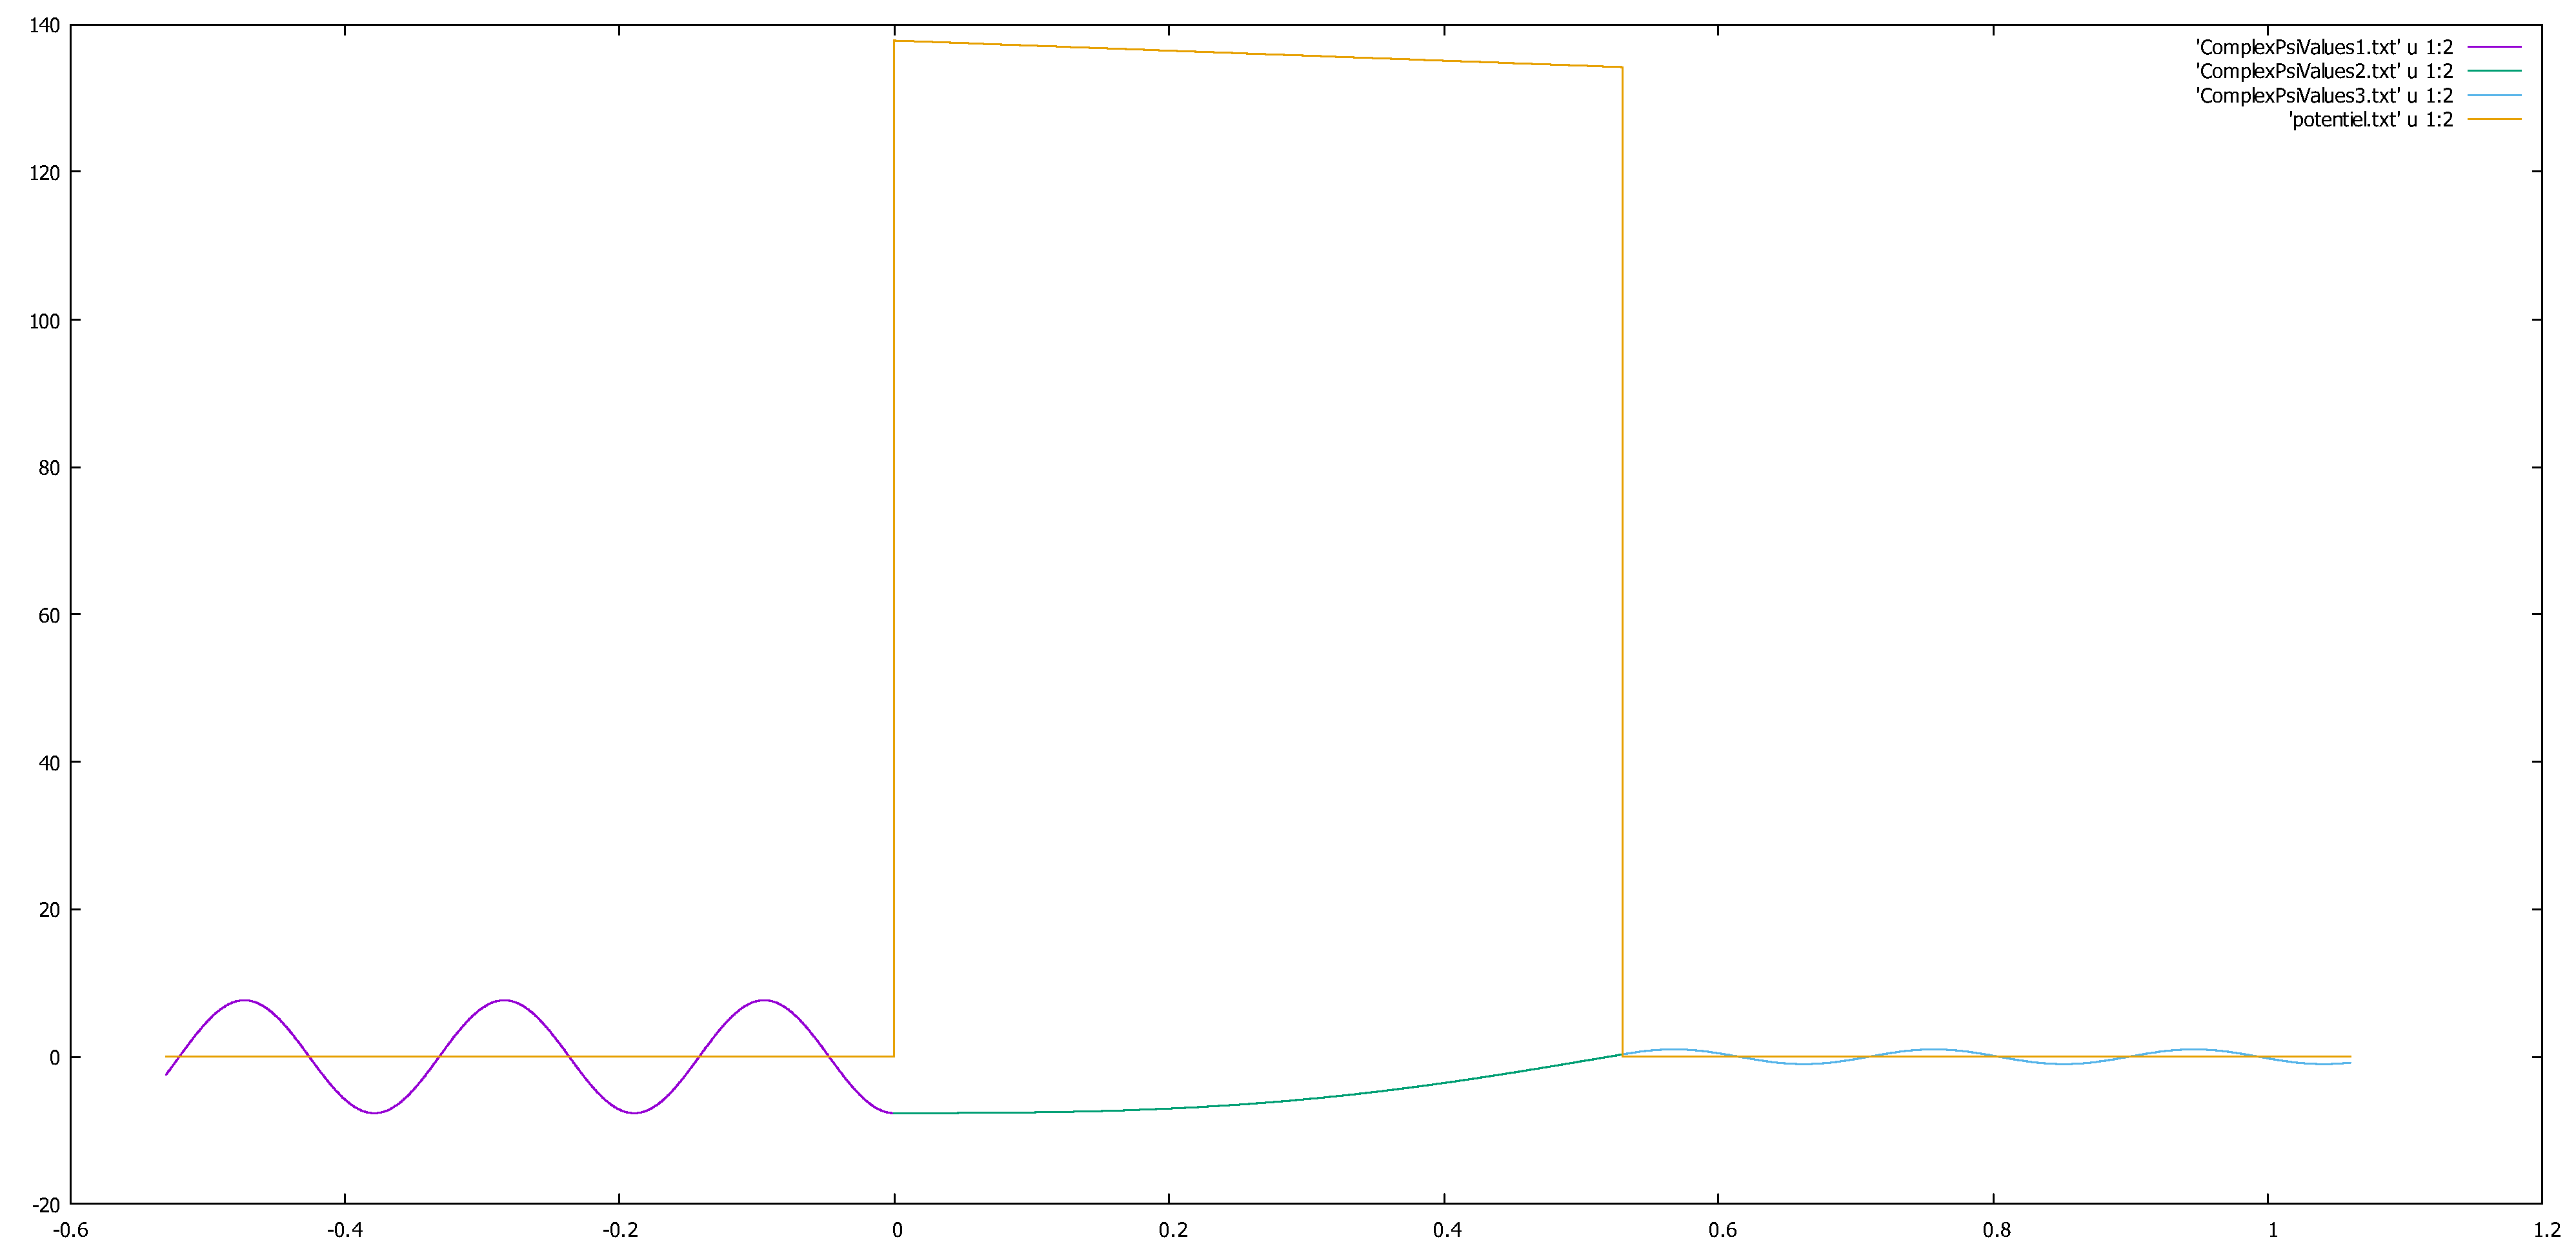
\includegraphics[width=0.4\textwidth]{Alpha/AlphaParticleDesintegration.pdf}
     \caption{Résolution Numérique de l'équation de Schrödinger pour une désintégration alpha}
     \label{fig:my_label}
 \end{figure}

\par En violet nous avons la courbe de l'onde en amont du potentiel et en bleu en aval de celle-ci.Nous observons le passage du fonction d'onde a travers le barrière en vert. Le coefficient de transmission pour cette application est calculé a T= 0.0632, d'où sur une grand nombre de phénomène de fission des particules traverse la barrière et sont émises. Le coefficient de réflexion quand a elle est de R= 0.9367.

\par Regardons a présent la courbe de Transmission en fonction de l'énergie du particule. 
\begin{figure}[!ht]
    \centering
    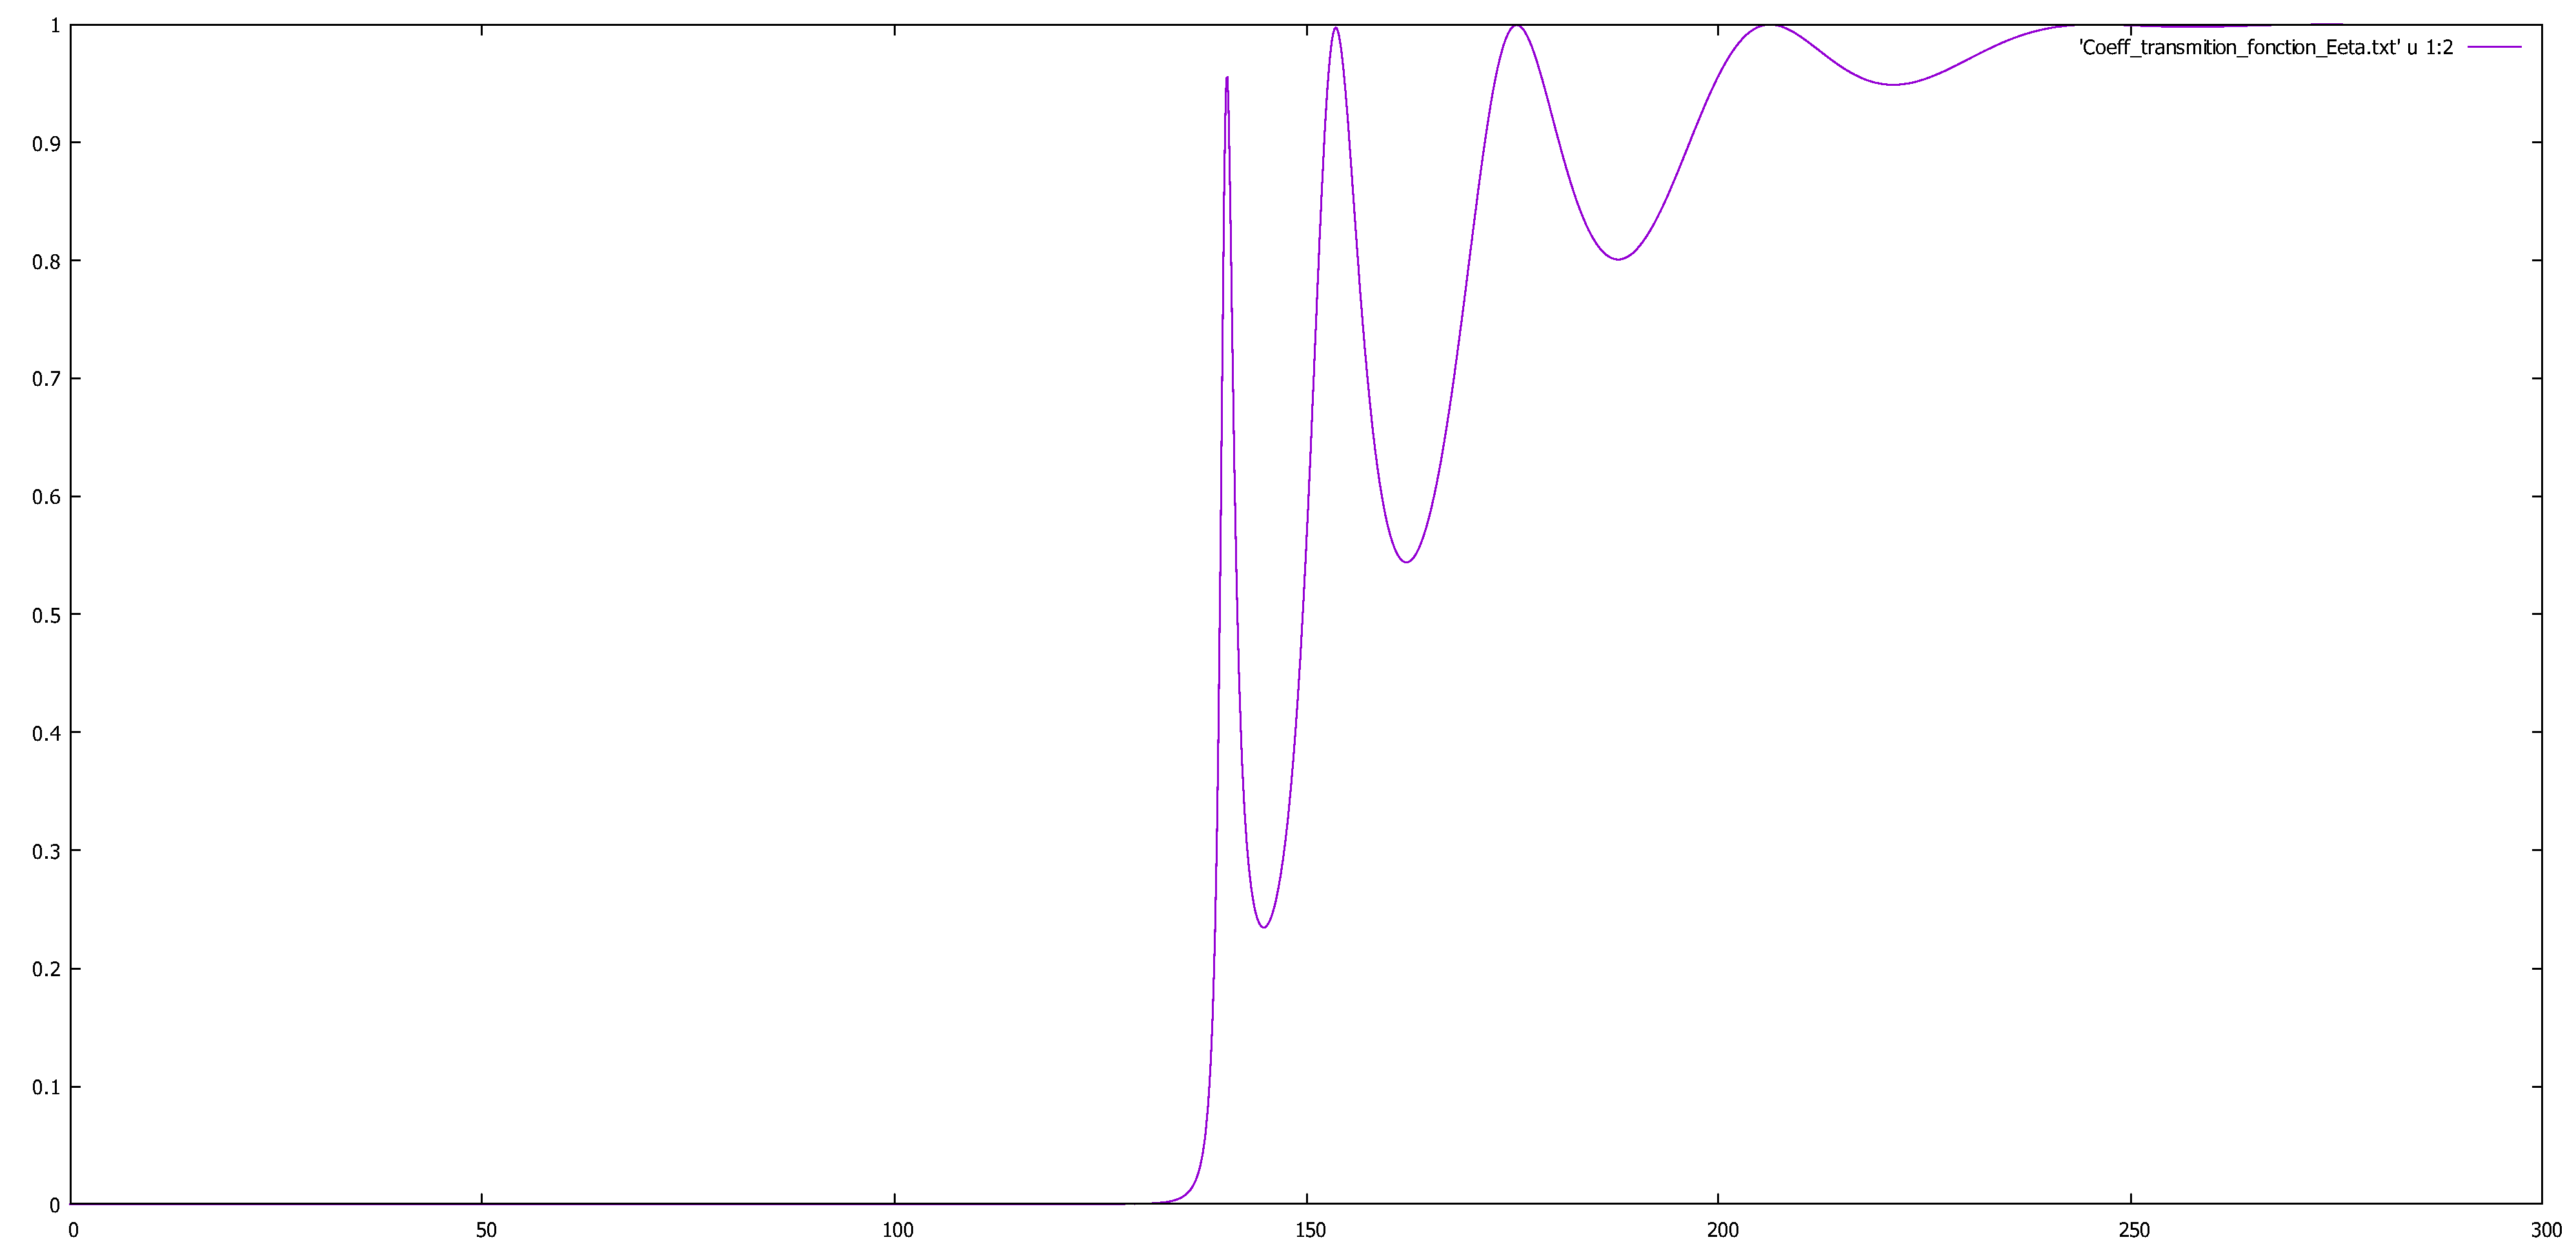
\includegraphics[width=0.4\textwidth]{Alpha/T(E).pdf}
    \caption{Coefficient de Transmission en fonction de l'énergie du particule alpha}
    \label{fig:my_label}
\end{figure}

Nous pouvons voir sur la fig.9, plusieurs valeur d'énergie pour lesquelles le coefficient de transmission est égale a 1 ou proche de 1. Pour observer ce qui se passe au niveau du premier pic, admettons les paramètres suivants:
\begin{table}[!ht]
\centering
Paramètres utilisés  $a=0.53$,\ $m=4.00151$,\ $V_{0}=140.56$,\ $N=10000$\\
\begin{tabular}{|l|l|l|}
\hline  Énergie & Coefficient de réflexion  & Coefficient de transmission \\
\hline  143.286 &  0.0787656025993423 &  0.921234397400658\\
\hline
\end{tabular}
\caption{Coefficients de réflexion et transmission}
\label{tab11}
\end{table}

\begin{figure}[!ht]
    \centering
    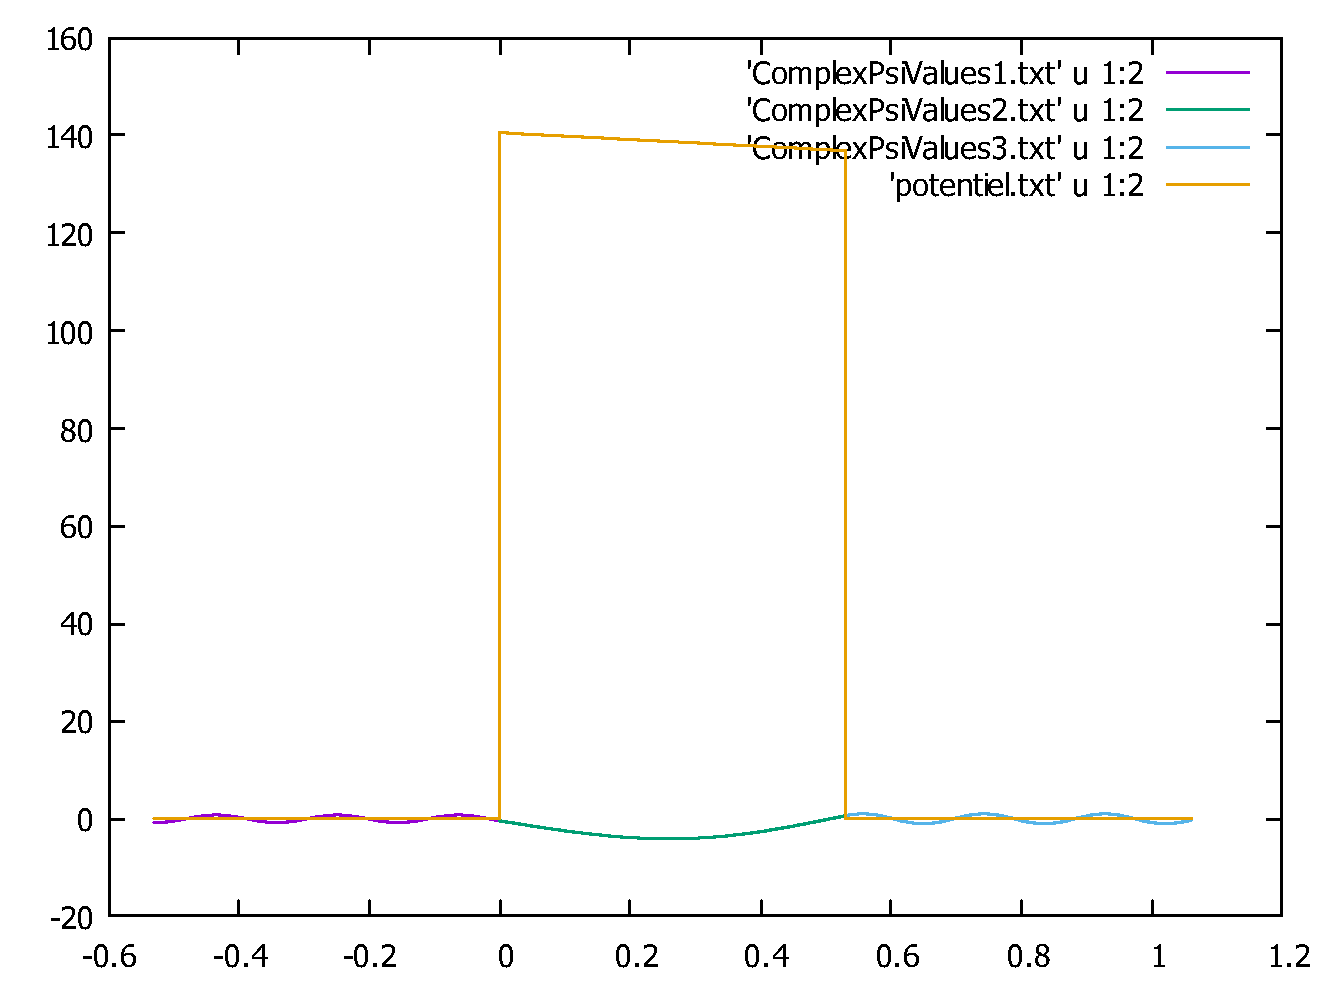
\includegraphics[width=0.6\textwidth]{AlphaResonnance/PsiReelResAplhaDecay.pdf}
    \caption{Capture du particule}
    \label{fig:my_label}
\end{figure}
\par Nous observons une particule en résonance avec le potentiel sur la figure 10. 

\subsubsection{Effet tunnel résonant}
\par L'effet tunnel est la capacité d'une particule quantique d'énergie inférieure a une seuil de franchir ce seuil. L'effet tunnel résonnant\cite{frwiki:182320873} quand a elle, apparaît lorsqu'une particule quantique aborde une tel système avec une énergie proche ou égale a celle du seuil. La probabilité de passage a travers les barrières est faible, mais la résonance avec le niveau des puits va piéger la particule, pendant une durée assez long, a l'intérieur du puits. Le coefficient de transmission de la particule est proche ou égale a l'unité dans ces instances. C'est pour cela que nous chercherons les résonances en observant la courbe de transmittivité en fonction de l'énergie lors de nos applications. 

\subsubsection{Capture de particule a travers une série de puits de potentiel}

\begin{table}[!ht]
\centering
Paramètres utilisés  $a=5$,\ $m=1$,\ $V_{0}=1$,\ $ N=20000 $\\
\begin{tabular}{|l|l|l|}
\hline  Énergie & Coefficient de réflexion  & Coefficient de transmission \\
\hline  0.47571 &  0.0202525776575487 &  0.979747422342451\\
\hline
\end{tabular}
\caption{Coefficients de réflexion et transmission pour une potentiel a 2 barrières}
\label{tab12}
\end{table}

\begin{figure}[!ht]
    \centering
    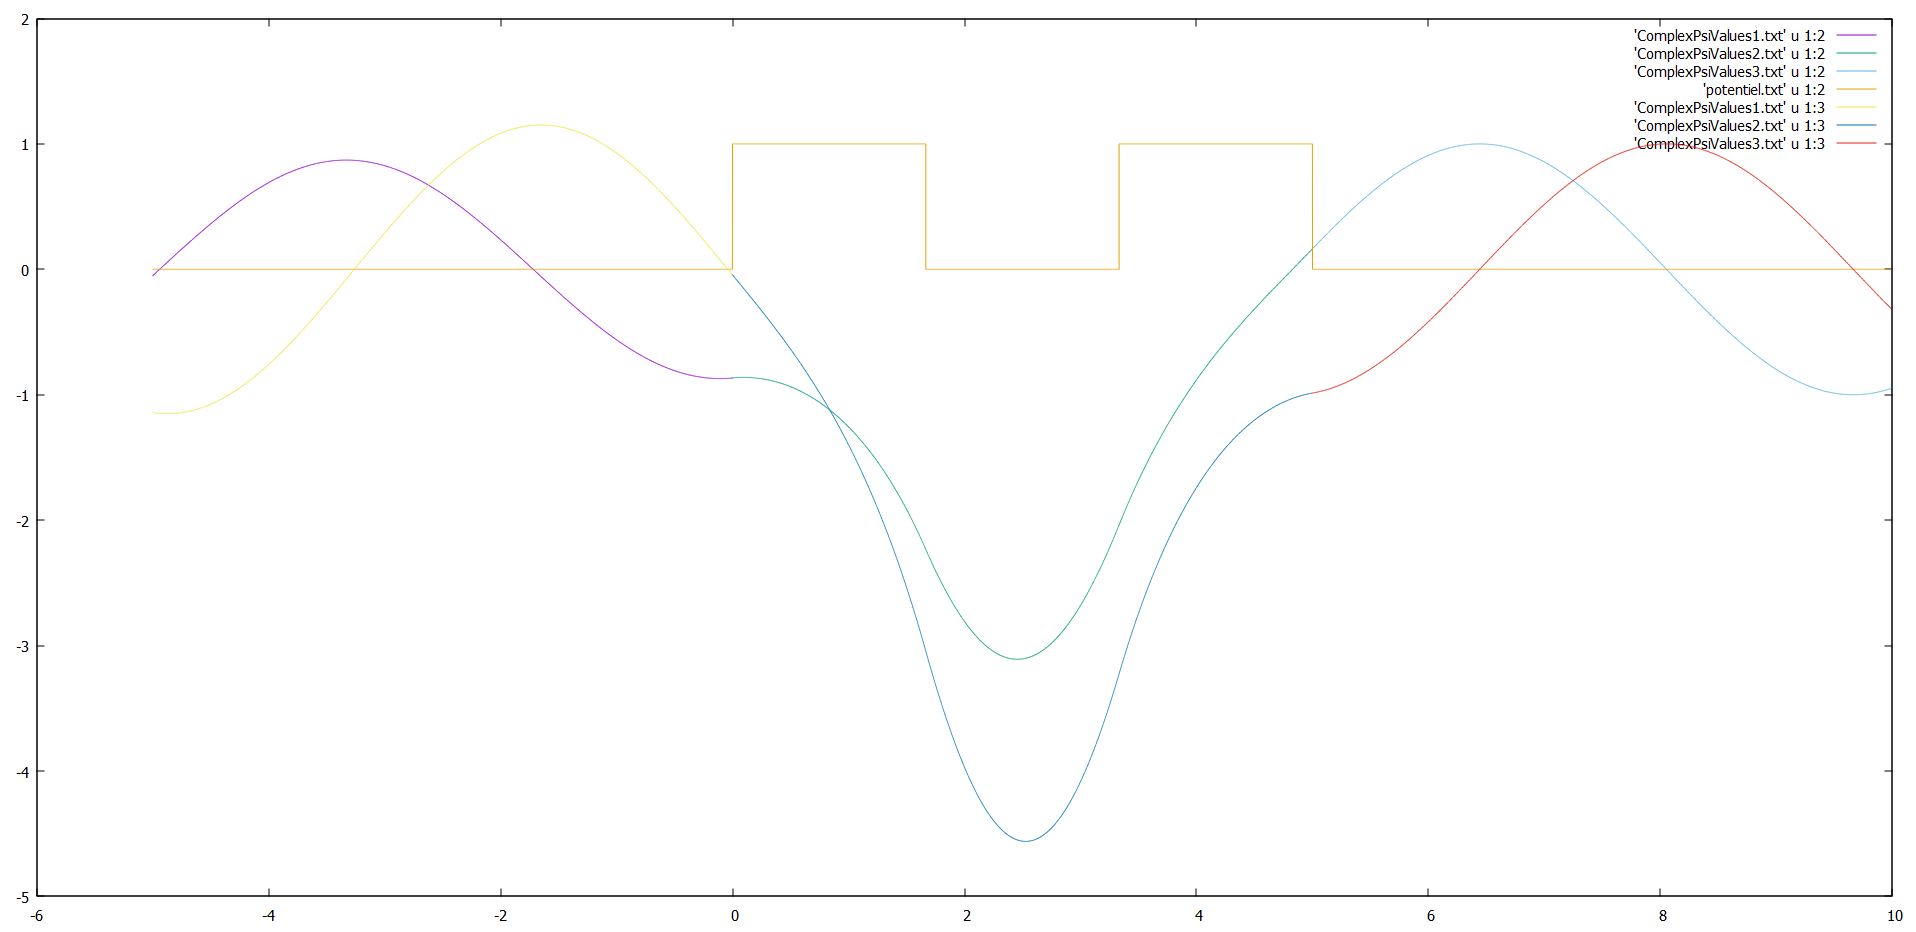
\includegraphics[width=0.8\textwidth]{2barriers Potentiel/2barReson.png}
    \caption{Capture du particule par 2 barrières de potentiel}
    \label{fig:my_label}
\end{figure}


\begin{table}[!ht]
\centering
Paramètres utilisés  $a=5$,\ $m=1$,\ $V_{0}=1$,\ $ N=20000 $\\
\begin{tabular}{|l|l|l|}
\hline  Énergie & Coefficient de réflexion 2 & Coefficient de transmission \\
\hline  0.606 &  0.0391264387378277 &  0.960873561262172\\
\hline
\end{tabular}
\caption{Coefficients de réflexion et transmission pour une potentiel a 3 barrières}
\label{tab12}
\end{table}

\begin{figure}[!ht]
    \centering
    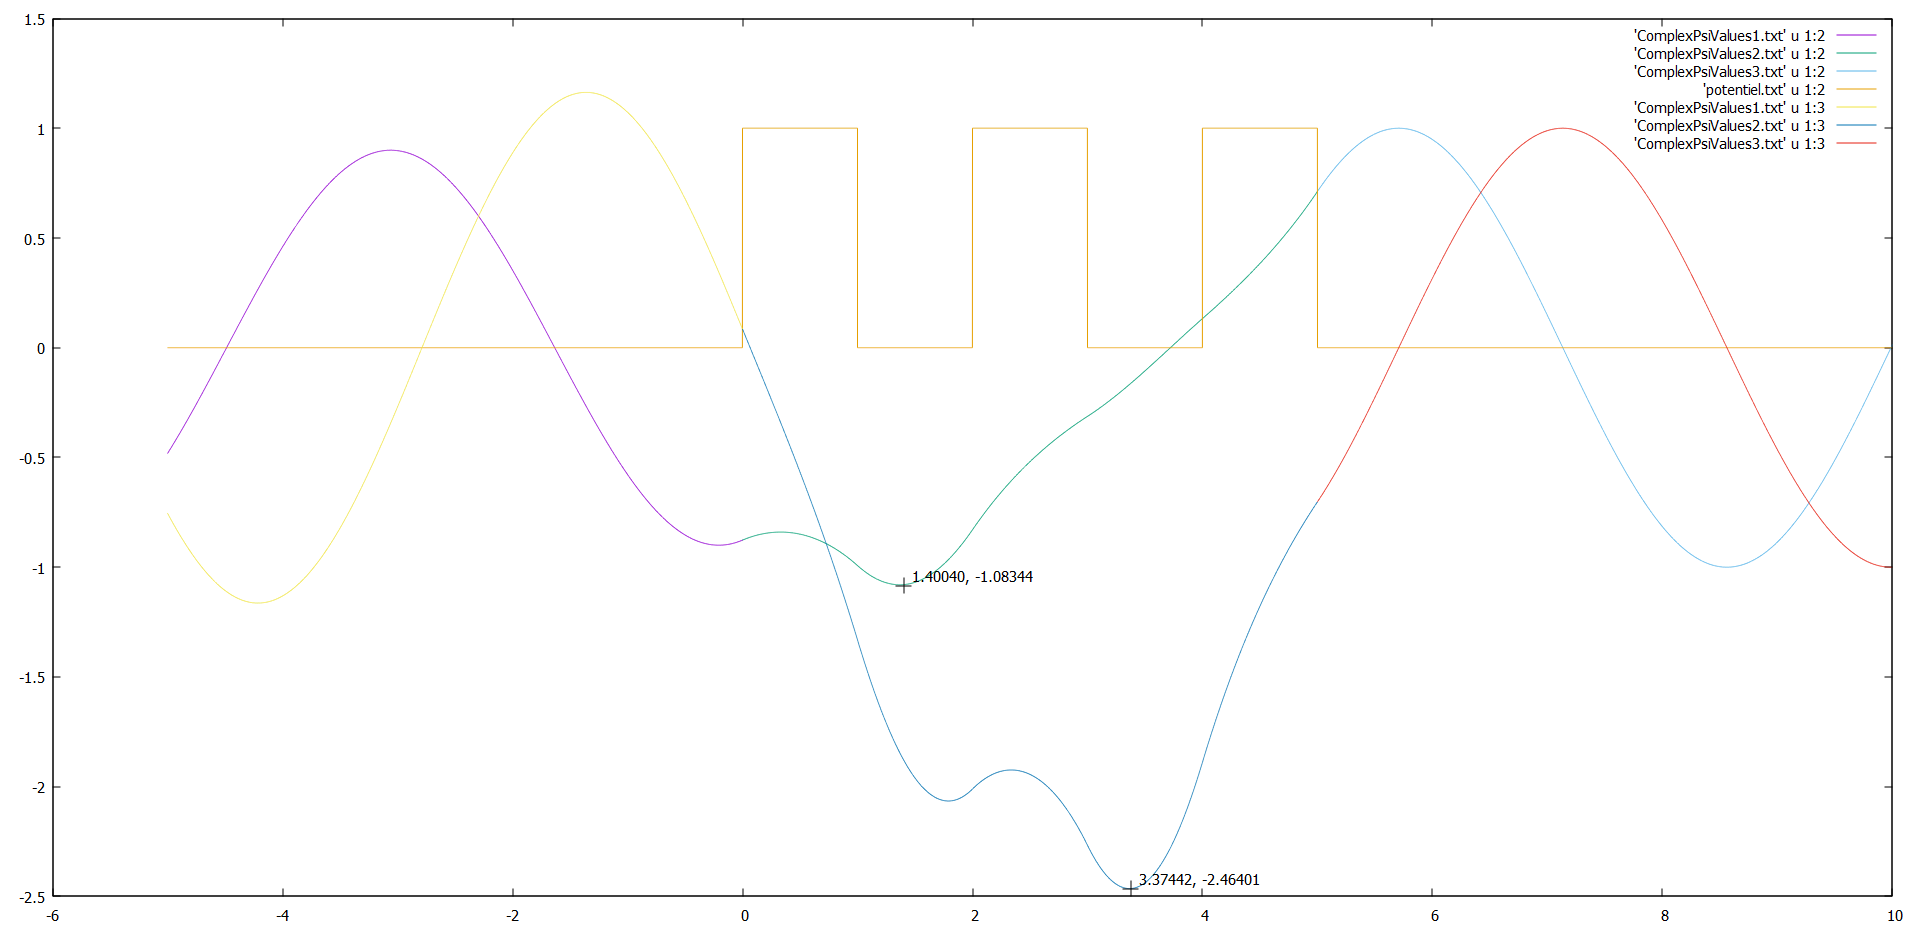
\includegraphics[width=0.8\textwidth]{3barriersResonnance/PsiReeletImaginaireReson.png}
    \caption{Capture du particule par 3 barrières de potentiel}
    \label{fig:my_label}
\end{figure}

\par Nous nous sommes positionné a la valeur de l'énergie de résonance, pour une série de puits de potentiel. 
\par Pour la fig. 11, nous remarquons que les parties réel et imaginaire de la fonction d'onde sont maximale et plus grand que le potentiel. La particule est bien capturée dans le puits démarqué par les deux barrières. 
\newpage
\par Pour la fig. 12, nous remarquons que la partie réel de la fonction d'onde est maximal est a l'unité au milieu du premier puits et que la partie imaginaire est maximal et plus grand que l'unité au niveau du second puits. En tenant en compte que le carré du fonction d'onde nous donne la densité de probabilité de présence du particule, nous pouvons en conclure que la particule est piégé au niveau du premier puits pour la plupart des réalisations de cette expérience.

\subsection{Variation de la taille du potentiel}

La variation du coefficient de transmission en fonction de la longueur du potentiel pour des énergies inférieurs à $V_{0}$. Pour une barrière de potentiel simple le coefficient de transmission sera décrit par la formule analytique \ref{eq:analityquee<v}. Si la condition $\alpha a >>1$ est vérifier le $sinh(\alpha a)$ va tendre vers $\frac{exp(\alpha a)}{2}$. Le coefficient de transmission va donc décroître exponentiellement.

\begin{center}
$T=\frac{16E(V_{0}-E)}{V_{0}^{2}}e^{-2\alpha a}$\\
paramètres utilisés $E=0.1$,\ $m=1$,\ $V_{0}=1$
\end{center}
\begin{figure}[!ht]
    \center
    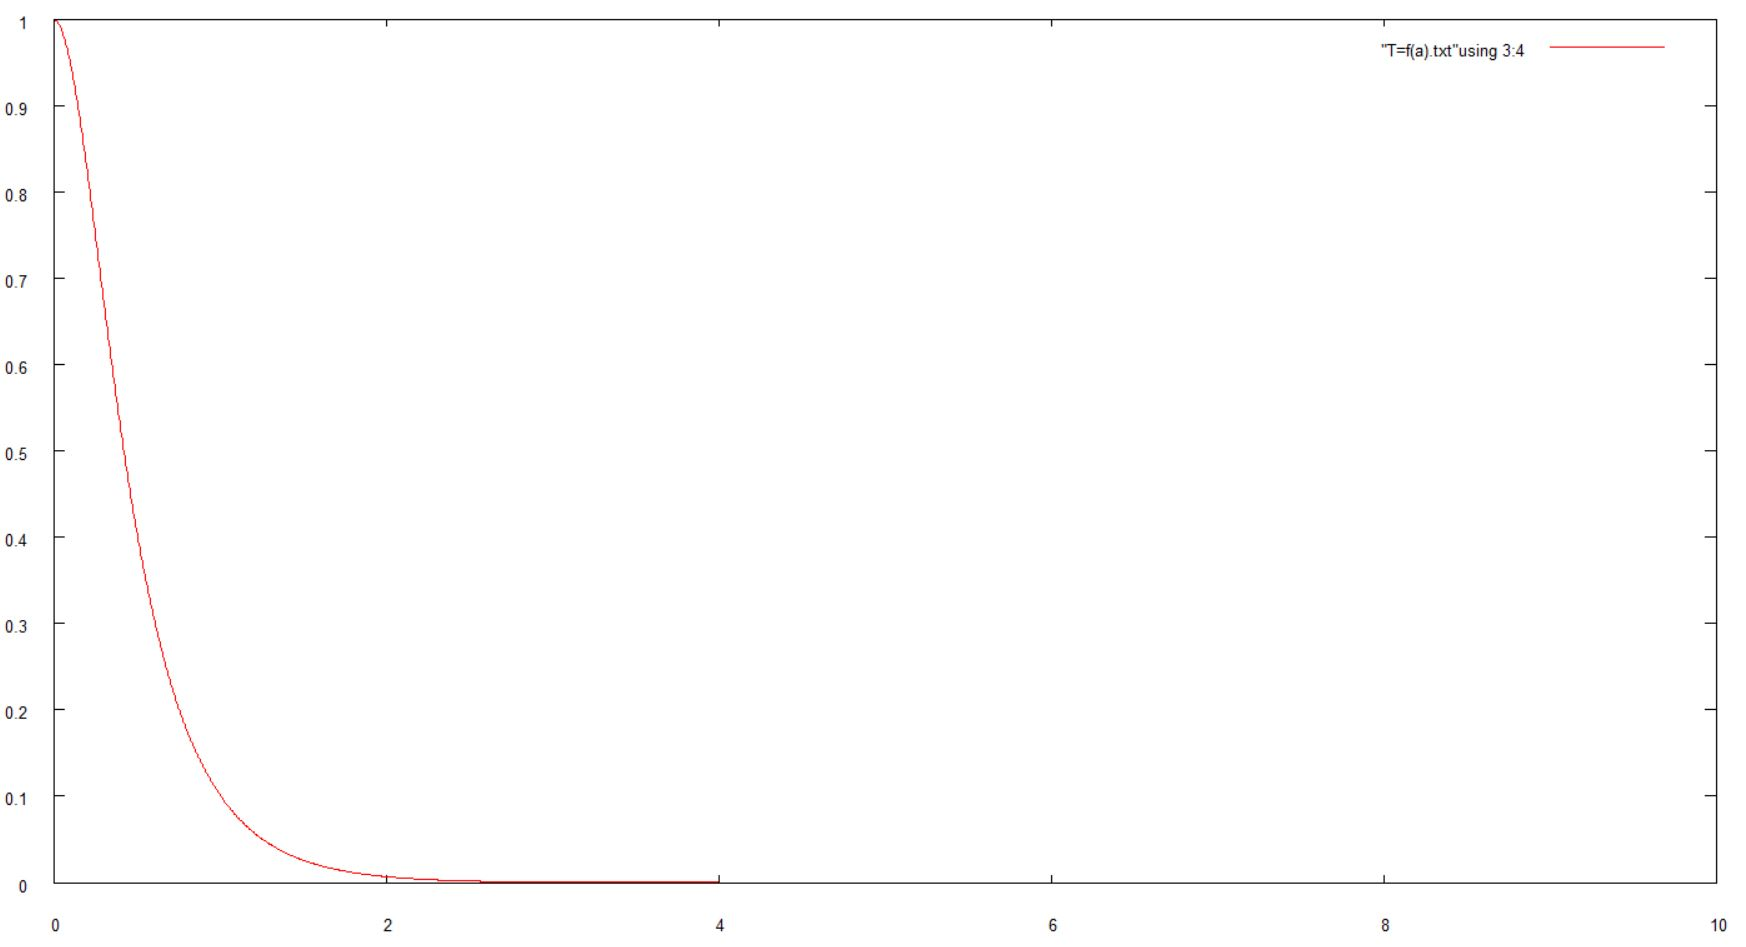
\includegraphics[width=0.5\textwidth]{t=f(a).jpg}
    \caption{Coefficient de transmission en fonction de x }
    \label{t=f(a)}
\end{figure}

Cette propriété de décroissance du coefficient de transmission est exploité par le microscope à effet tunnel. Le principe du STM  (scanningtunneling microscope) est d'approcher une pointe de la surface que l'on veut cartographier, la distance entre la pointe et la surface peut être assimiler à une barrière de potentiel. Lorsque l'on est suffisamment  proche on détecte un courant qui est transmit par effet tunnel. Le courant va suivre la même décroissance que le coefficient de transmission se qui permet d'avoir des résolutions de la surface inférieur à la taille d'un atome.



\subsection{Variation de la masse}

\begin{figure}[!ht]
    \centering
    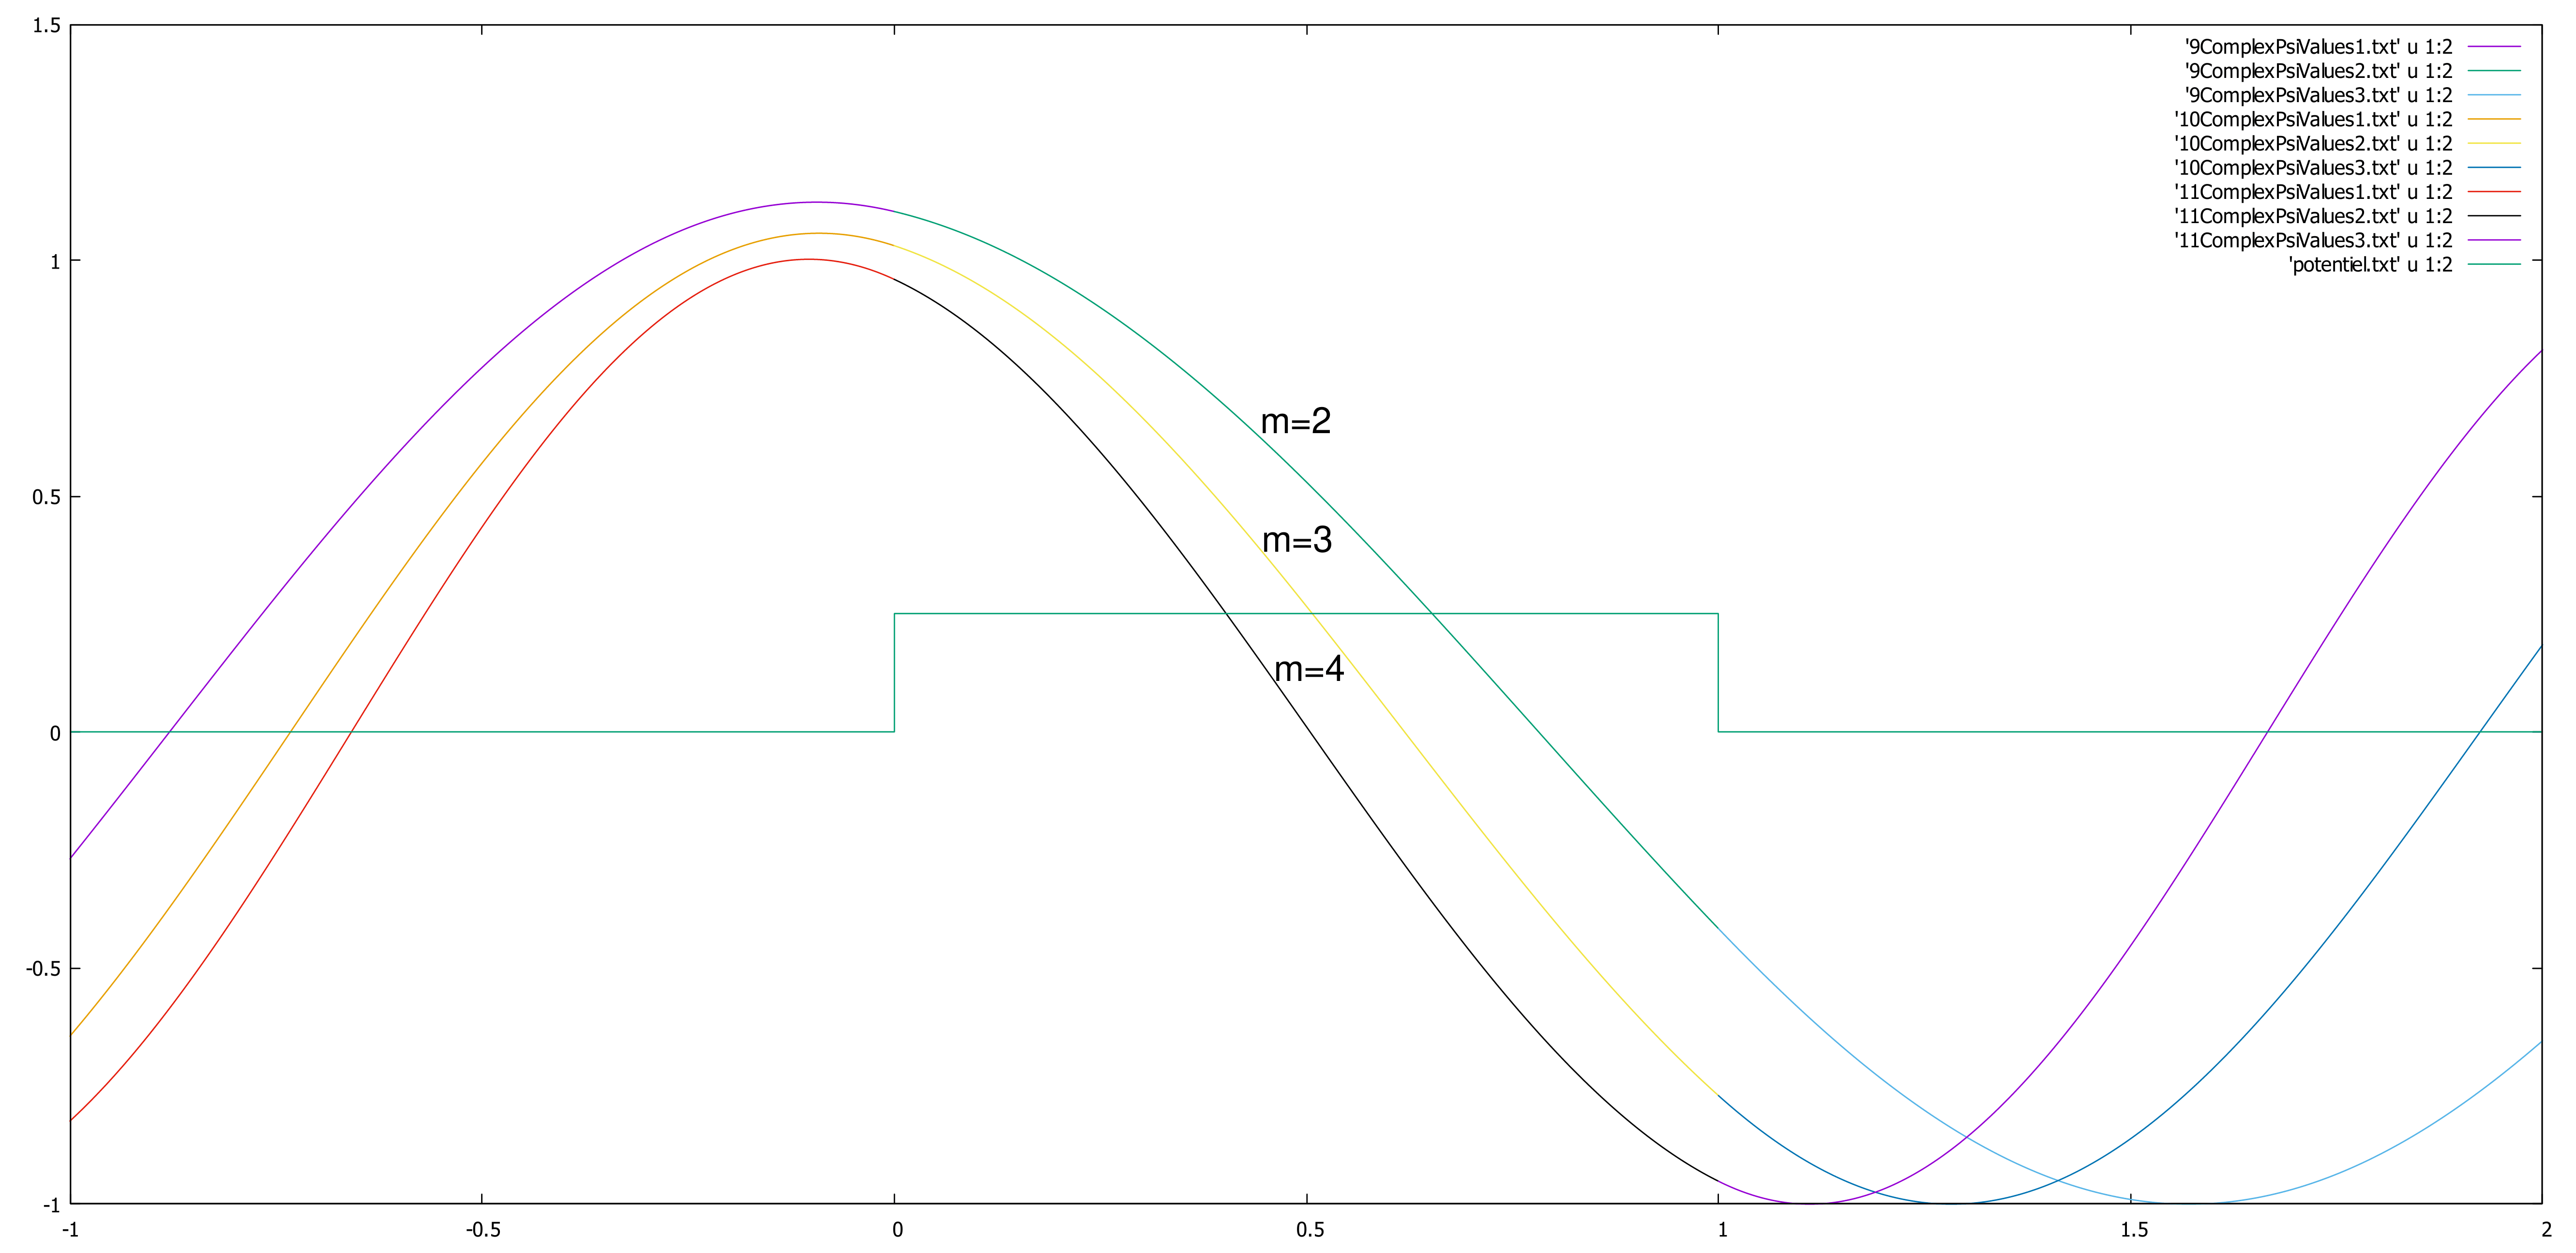
\includegraphics[width=0.8\textwidth]{potentiel 1 barrier/m augmentant seul2-1.png}
    \caption{Partie réel de $\Psi$(x) avec m comme paramètre fluctuant}
    \label{fig:my_label}
\end{figure}

\begin{table}[!ht]
\centering
Paramètres utilisés $E=1$,\ $a=1$,\ $V_{0}=0.25$,\ $N=20000$\\
\begin{tabular}{|l|l|l|}
\hline  masse & Coefficient de réflexion  & Coefficient de transmission \\
\hline  2 & 0.0198908911855625 &  0.9801091104902894\\
\hline 3 & 0.014900596680466 & 0.985099405784575\\ 
\hline 4 & 0.00840550290054031&0.991594500394001\\
\hline
\end{tabular}
\caption{Coefficients de réflexion et transmission}
\label{tab}
\end{table}